\newcommand{\institut}{Institut f\"ur Telekommunikationssysteme}
\newcommand{\fachgebiet}{Nachrichten\"ubertragung}
\newcommand{\veranstaltung}{Praktikum Nachrichten\"ubertragung}
\newcommand{\pdfautor}{Dirk Babendererde (321 836), Thomas Kapa (325 219)}
\newcommand{\autor}{Dirk Babendererde (321 836)\\ Thomas Kapa (325 219)}
\newcommand{\gruppe}{Gruppe:}
\newcommand{\betreuer}{Betreuer: Lieven Lange}


\newcommand{\pdftitle}{Nachrichtenuebertragung\ Praktikum\ 05}
\newcommand{\prototitle}{Praktikum 05 \\ Pulsamplitudenmodulation und nichtideale Abtastung}

\input{../../packages/tu_header_9}

% damit das outline funktioniert noch mal:
\begin{document}


%     \lstinputlisting{./praktikum6.sce}

%---------------------------------------------------------------------
%---------------------------------------------------------------------
%---------------------------------------------------------------------

\section{Vorbereitung}
\begin{quote}
    
    
    \begin{figure}[H]
        \centering
        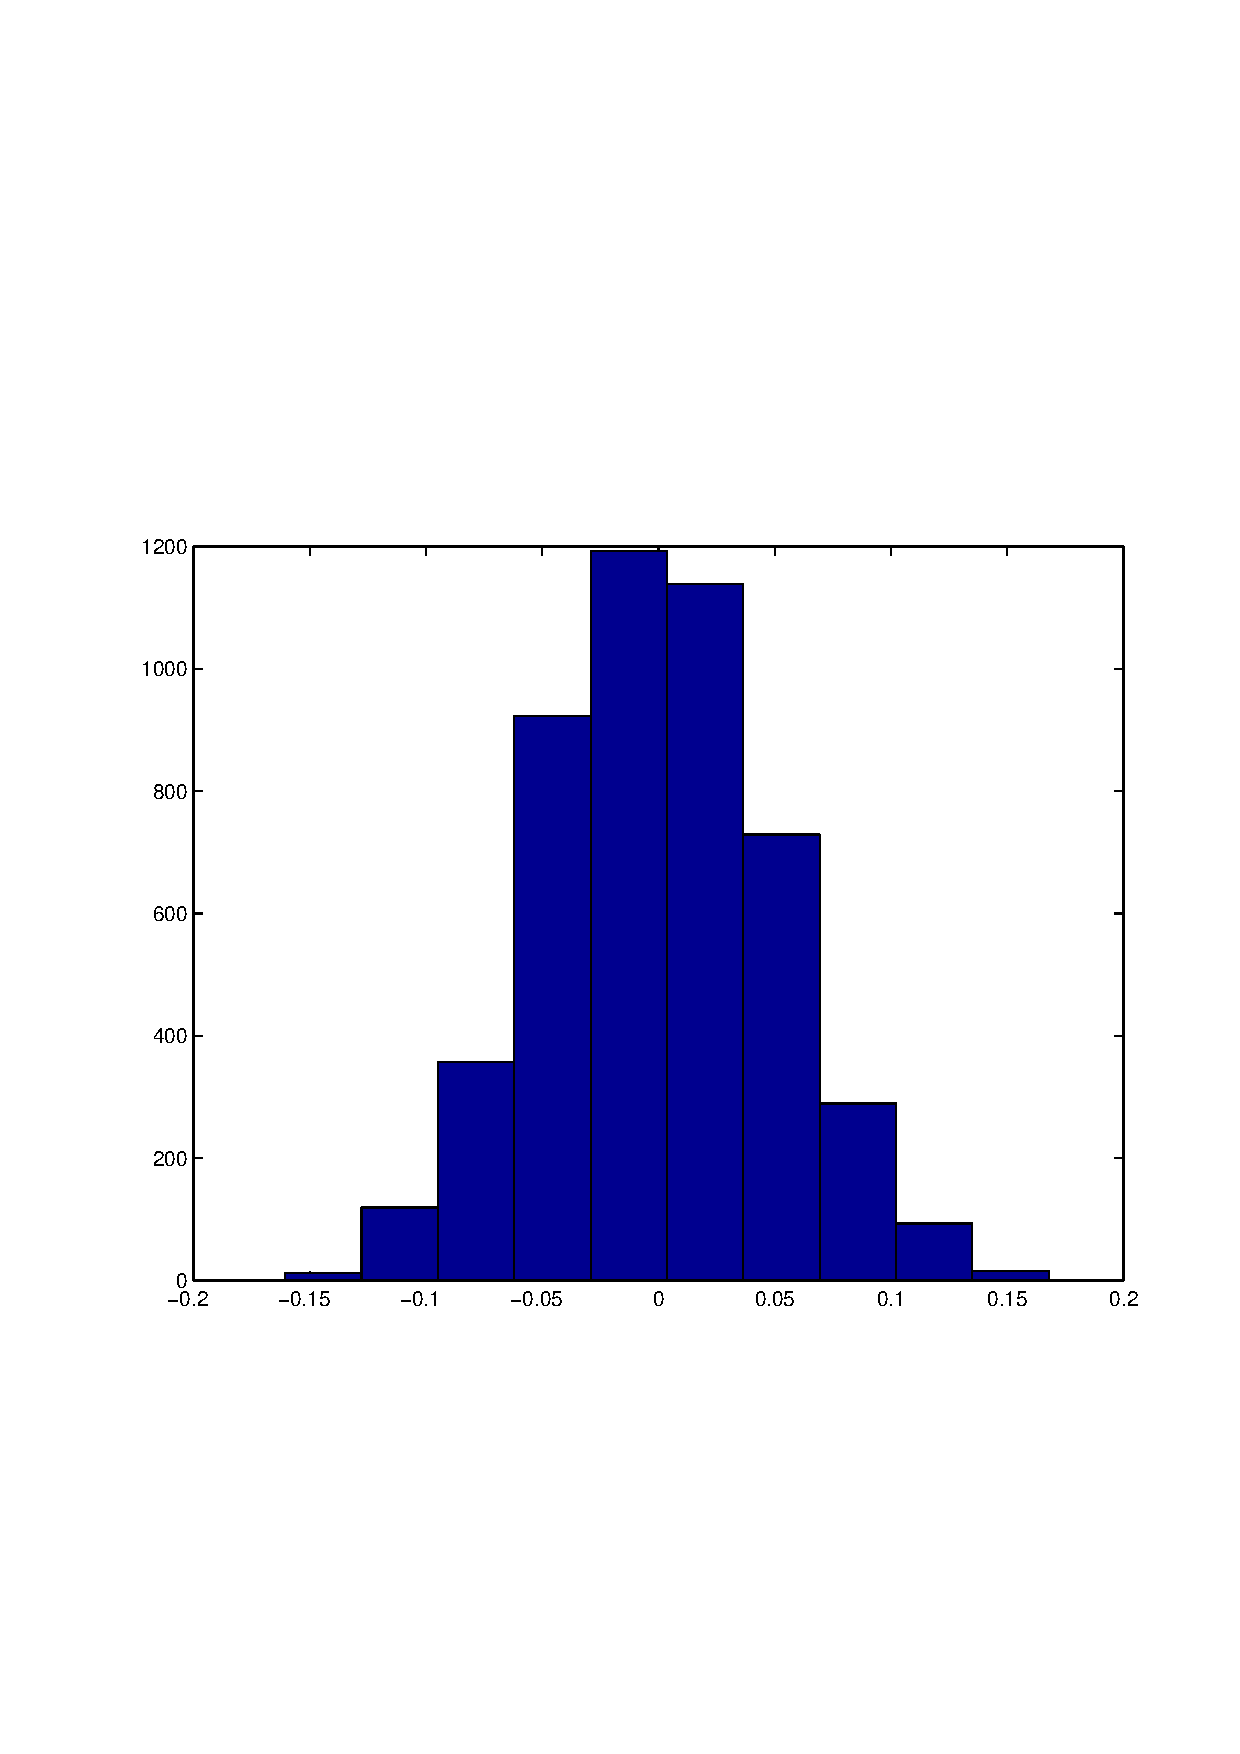
\includegraphics[scale=0.7, trim = 2cm 7cm 1cm 8cm, clip]{Bilder/PCM_Test}
        \caption{Testkennlinie des PCM-Analyse Scriptes}
        \label{fig:PCM_Test}
    \end{figure}
    
    
    \TODO{Blockschaltbild? erklärung?}
    
    
    
    
\end{quote}


\section{Labordurchführung}
\begi{quote}

	Es soll die PCM-Encoder-Kennlinie aufgenommen werden.
	Dazu wird das PCM-Encoder-Modul des ETT101 genutzt. Zunächst wird als Clocksignal an den Eingang CLK das 
	100 kHz DIGITAL Signal des Master Signals-Modul gelegt. Anschließend wird als Eingang in INPUT 1 ein 
	symmetrisches Dreiecksignal mit einer Amplitude von 2,5 Volt angelegt (2,5 Volt, damit für über 2 und unter -2 Volt die
	Codewörter 1111 1111 und 0000 0000 ausgegeben werden). 
	Die beiden Ausgänge FS (Rahmensignal) und PCM (Pulsecode) werden auf die beiden Eingänge des Addierers gegeben. Da
	beide Signale 5 Volt high und 0 Volt low ausgeben, wird die Verstärkung für das PCM-Signal auf 0 gestellt und die
	Verstärkung für das Rahmensignal auf 8/5 gestellt, um die Anforderungen aus der Aufgabenstellung zu erfüllen.
	Um 
 	
	
	
\end{quote}

\section{Auswertunf \& Theorie}
\begin{quote}
    
\end{quote}






\end{document}